\section{使用一个模板}
{\BIThesis} 整个项目中包含多个模板,每个模板各自位于独立的文件夹中。

\subsection{熟悉简单 \LaTeX 语法}
如果你之前没有接触过 {\LaTeX},请前往 Overleaf 的“\href{https://www.overleaf.com/learn/latex/Learn_LaTeX_in_30_minutes}{30 分钟学习 {\LaTeX}}”文档进行阅读,从而对 {\LaTeX} 有大致的印象。

一些常用的 {\LaTeX} 格式与使用技巧:

\begin{itemize}
  \item \href{https://www.overleaf.com/learn/latex/Sections_and_chapters}{{\LaTeX} 章节设定:Sections and chapters}
  \item \href{https://www.overleaf.com/learn/latex/Paragraphs_and_new_lines}{{\LaTeX} 段落格式:Paragraphs and new lines}
  \item \href{https://www.overleaf.com/learn/latex/Bold,_italics_and_underlining}{{\LaTeX} 粗体、斜体与下划线:Bold, italics and underlining}
  \item \href{https://www.overleaf.com/learn/latex/Lists}{{\LaTeX} 有序列表、无序列表:Lists}
  \item \href{https://www.overleaf.com/learn/latex/Inserting_Images}{{\LaTeX} 插入图片:Inserting Images}
  \item \href{https://www.overleaf.com/learn/latex/Tables}{{\LaTeX} 构建表格:Tables}
  \item \href{https://www.overleaf.com/learn/latex/Mathematical_expressions}{{\LaTeX} 插入数学公式:Mathematical expressions}
  \item \href{https://www.overleaf.com/learn/latex/Code_Highlighting_with_minted}{{\LaTeX} 插入代码与代码高亮:Code Highlighting with minted}
  \item \href{https://www.overleaf.com/learn/latex/algorithms}{{\LaTeX} 插入算法伪代码描述:Algorithms}
  \item \href{https://www.overleaf.com/learn/latex/Bibliography_management_in_LaTeX}{使用 {Bib\LaTeX} 管理参考文献:Bibliography management in LaTeX}
\end{itemize}

有关 {\LaTeX} 使用的更多技巧,请直接前往 \href{https://www.overleaf.com/learn/latex/Main_Page}{Overleaf 官方文档}进行查看。准备就绪之后,你就可以前往下载 {\BIThesis} 模板啦。

\subsection{在项目的 Release 页面下载你希望使用的模板}
为了方便各位同学使用,项目按照 Release 发布的流程,将每个模板进行打包,并在每次发版后用 GitHub Release 进行模板分发。也就是,你可以直接前本项目的 GitHub Release 页面,直接下载你所希望使用的模板压缩包,并解压到本地进行使用。

你可以点击这个链接前往最新的 Release 版本进行模板下载:

\begin{center}
  \color{ForestGreen}\href{https://github.com/spencerwooo/BIThesis/releases/latest}{https://github.com/spencerwooo/BIThesis/releases/latest}
\end{center}

在 Release 页面,你会看到:

\dirtree{%
.1 /.
.2 proposal-report.zip \ldots{} \color{RoyalBlue}{本科生毕业设计开题报告模板压缩包}.
.2 graduation-thesis.zip \ldots{} \color{RoyalBlue}{本科生毕业设计毕业论文模板压缩包}.
.2 lab-report.zip \ldots{} \color{RoyalBlue}{本科生实验报告模板压缩包}.
}

\begin{figure}[H]
  \centering
  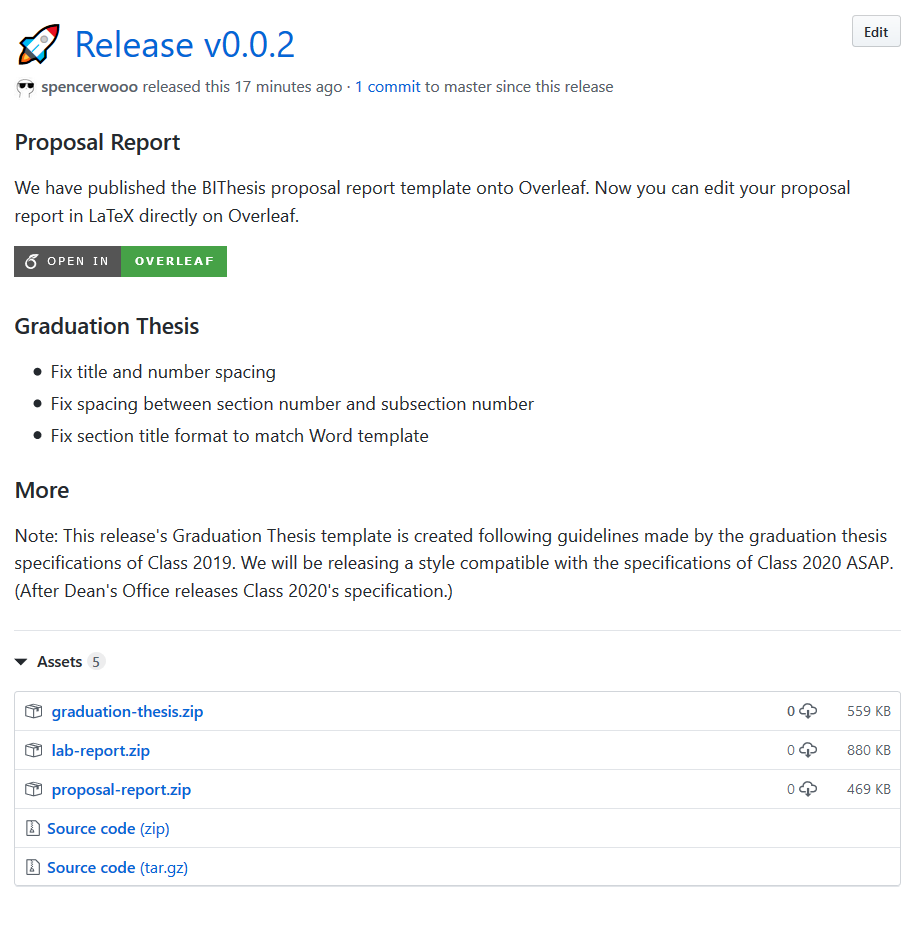
\includegraphics[width=\textwidth]{images/release.png}
  \caption{{\BIThesis} 的 Release 页面}
\end{figure}

根据你的选择,下载其中你所要使用的模板即可。(当然,你也可以直接用 Git 将本项目完整克隆至本地,使用最新版本的模板。)
